% This is lnicst.tex the demonstration file of the LaTeX macro package for
% Lecture Notes of the Institute for Computer Sciences, Social-Informatics 
% and Telecommunications Engineering series from Springer-Verlag.
% It serves as a template for authors as well.
% version 1.0 for LaTeX2e
%
\documentclass[lnicst]{svmultln}
%
\usepackage{graphicx} % includegraphics
\usepackage{makeidx}  % allows for indexgeneration
% \makeindex          % be prepared for an author index
%
\begin{document}
%
\mainmatter              % start of the contribution
%
\title{Obfuscation with Turing Machine}
%
\titlerunning{Hamiltonian Mechanics}  % abbreviated title (for running head)
%                                     also used for the TOC unless
%                                     \toctitle is used
%
\author{Yan Wang\inst{1} \and Dinghao Wu,\inst{2}
Shuai Wang \and Pei Wang}
%
\authorrunning{Ivar Ekeland et al.}   % abbreviated author list (for running head)
%
%%%% list of authors for the TOC (use if author list has to be modified)
\tocauthor{Ivar Ekeland, Roger Temam, Jeffrey Dean, David Grove,
Craig Chambers, Kim B. Bruce, Elisa Bertino}
%
\institute{Pennsylvania State University, State College,PA 16801, USA,\\
\email{ybw5084@ist.psu.edu},\\ WWW home page:
\texttt{http://users/\homedir iekeland/web/welcome.html}
% \and
% Universit\'{e} de Paris-Sud,
% Laboratoire d'Analyse Num\'{e}rique, B\^{a}timent 425,\\
% F-91405 Orsay Cedex, France}
}
\maketitle              
% typeset the title of the contribution
% \index{Ekeland, Ivar} % entries for the author index
% \index{Temam, Roger}  % of the whole volume
% \index{Dean, Jeffrey}

\begin{abstract}        % give a summary of your paper
Software security is a fundamental research domain in this threat emerging technology world. Leveraging system vulnerbilities is one of the common ways to hack into 
computer system. Hackers have to understand the program control flow in order to figure out the hacking logic and technique. In this way, consealing important branch trigger condition logics are crucial for protecting softwares from being hacked. In this paper we propose a novel control flow obfuscation method with Turing machine. By entwining the original software programs with Turing machine executio, software control flow graphs could be significantly obfuscated which means it is much more harder or even impossible for hackers to embed malicious execution codes into Turing machine obfuscated programs.We implemented a obfuscation tool to gernerate obfuscated binaries using LLVM. Evaluation results demonstrate that software programs become much more complicated after Turing maching obfuscation. At current stage, we only obfuscated the interger operand instructions which are vital to the whole program.
%                         please supply keywords within your abstract
\keywords {software security,control flow obfuscation, Turing machine,LLVM}
\end{abstract}
%
\section{Introduction}
%
Obfuscation derives from intellectual property protection. Internet brings us unprecedent convience and threat of idea plagiarism and copyright infringement at the same time.  Consealing the algorithm of a software means a lot for the society especially for high-tech industry. Reverse engineering is often used by to recover source code from binaries to analyze software vulnerbilities or to steal software ideas or algorithms. Obfuscation is a technique to block or harden the process of reverse engineering.

Recently, Software security has become a bigger and bigger concern in research community because of infamous ransomware attack and severe vulnerbiliy such as the recent ``Wanncry'' insidence and the openssl heartbleeding bug.This incidences challenge the computer world greatly. Hackers endevors to figure out vulnerbilities inside a software program. Knowing the software architecture and program logic like control flow graph is an indispensible prerequisite for hackers to analyze the original codes. With the help of some monitoring techniques hackers could even iterate all possible paths to try to restore all important branch information along the execution paths.\textit{Concolic testing} is an example which expoits symbolic execution given a certain input while it keeps changing input data until the code coverage proceed a threshhold\cite{Sen} as shown in Figure 1. It has been proved to work in restoring the branch information in the original source codes. Hence, a lot of research focus on preventing bad guys from figuring out the essential logic. Consealing important ``crossroad'' in a source program. Control flow obfuscation is one of these techniques. Control flow obfuscation aims at hiding conditional transfers and complicating the execution path within a source program. Through replacing or insering extra contrlo flow graph edges, the original software logic become harder or even impossible to trace. Previous research\cite{Ma} have prove the effectiveness of contral flow obfuscation.

\begin{figure}
  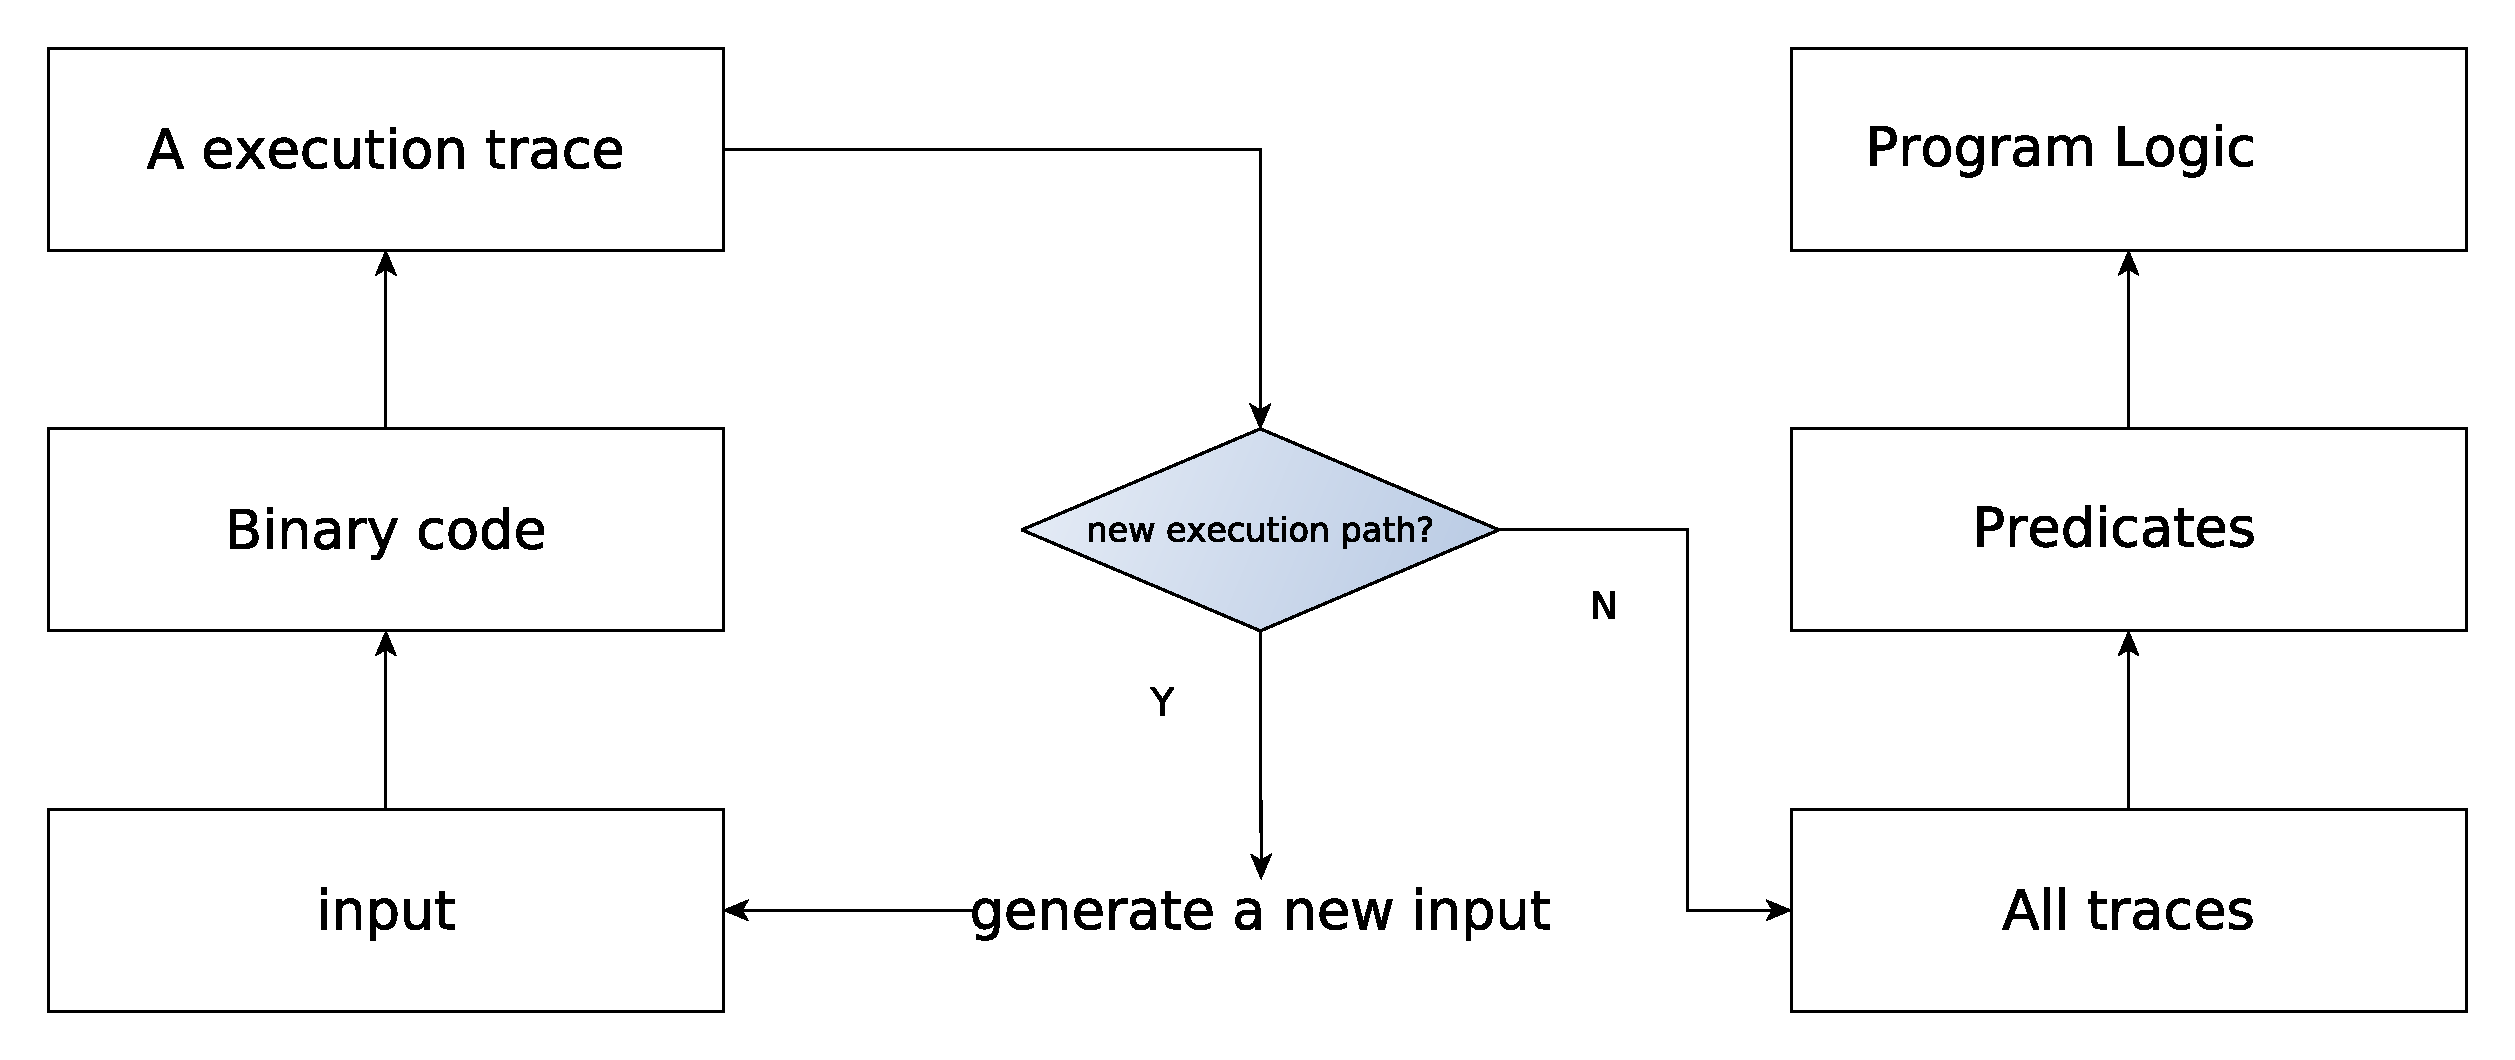
\includegraphics[width=0.9\linewidth]{reverse_engineering.eps}
  \caption{Reverse engineering with concolic testing}
  \label{Figure 1}
\end{figure}

In this paper,we propose a novel control flow obfuscation method with Turing machine embedded in the original program source codes. Turing machine is the essence of computaion so it could calculate accurately all kinds of computer operation. In this way, important branch conditions in original source code could be replaced by a Turing machine execution which yields the very identical conditional value. Besides, a Turing machine behaves like a state machine so it contains a lot of branch condition checks in Turing machine transition table. In this whole process, sensitive branch information could be successfully hided in Turing machine call graphs. In the mean time, Turing machine execution greatly introduce computational complexity to the target program so it is almost impossible to read the obfuscated programs to do reverse engineering. 

Currently, we are more interested in integer operation condition instructions. Utilizing LLVM, we could turn original program source codes into intermediate representation(IR).Turing machine obfuscator take over from IR and select interested instruction candidates which would be redirected to semantic equivalent Turing machine execution. After all paths finished in the Turing machine ``blackbox'', the original call graph resumes from the the obfuscator interrupt and the whole program control flow graph is greatly expanded and complicated. Since LLVM is the implementation foundation, currently our proposed obfuscator could only be applied to C/C++ source programs. Inspired by previous previous works\cite{Collberg},we evaluate our obfuscator from four demensions which are potency,resilence, cost and stealth respectively. Results indicates that Turing machin obfuscator could effectively obfuscate target source codes with acceptable cost overhead.

This paper is organized as follows. Section 2 discusses related works on obfuscation, especially control flow obfuscation. Section 3 illustrate the idea and archetecture of Turing machine obfuscator. Obfuscator implementation is discussed in section 4. Section 5 discusses the evaluation result of our proposed obfuscator. Finally, we conclude thsi paper in section 6.


%
\section{Related Works}
%
Generally speaking, reverse engineering is devided into static analysis such and dynamic analysis. To compete static reverse engineering, researchers usually focus on hardening disassembling and decompiling process. To compete the dynamic reverse engineering techniques such concolic testing, conditional transfer logic must be hidden from adversaries. Control flow obfuscation has been proved effective in previous works.

In \cite{Sharif}, the authors identified conditions that could trigger malware execution then using hash function to transform the values which could launch malware. Afterwards, correspondent conditional codes which would be ran with satisfied value were encryped with a key generated based on the instruction trigger value.
By this means the obfuscation analyzer could never get a chance to get the expected ``launching code'' consequently planted malware could never be executed. This technology works on certain fixed trigger value but not in senarios that trigger values are intervals such as \textgreater \   and  \textless. This limitation narrows the applicable conditions greatly since a large volume of branch conditions are comparsion operations. In addition, the encrytion and decryption process in this methodology also introduce inneglectable overhead.

In \cite{Popov}, the authors used signals(``traps'') to replace the control transfers unconditional instructions like ``jmp'' and ``call'' in order to confuse disassembly operation which is the first step of reverse engineering. Dummy control transfers and junk instructions were also inserted after signal replacements. This method seems to be effective in fooling disassemblers but it can't be applied in senarios that conditional instruction logic needs to be protected from being figured out.

In \cite{Zhi}, the authors endevors to conseal branch information leveraging a remote trusted third party environment. The idea seemed to work while it not only introduced a great network overhead, but also rely on trusted network accessiblity which can't be guranteed in reality. This drwaback means this idea can't be applied in common obfuscation cases.

In \cite{Ma}, the authors took advantage of neural network to replace appropriate conditional instructions in source programs in order to achieve the goal of consealing conditional instruction logic thus dynamic analysis like concolic testing could never dig useful branch information. Although the idea looks promising and the results indicates the effectiveness of this methodology to some degree, fundamentally we don't believe neural networks solution is suitable for such senarios. To the best of our knowledge,
neural networks works like a blackbox. It lacks the rigorous mathmatical proof to illustrate a correct result must be generated given a input. Neural networks not only introduced complexity but also unpredictability to the original source programs. Trained models may behave very differently if given initial parameters with only some nuances, which means that it is also very hard to train a accurate enough model to simulate the conditional instruction. In addition, we noticed that neural networks consume too much memory in the evaluation experiments.

%
\section{Turing machine obfuscation overview}
%
We assume that $H$ is
$\left(A_{\infty},B_{\infty}\right)$-sub\-qua\-dra\-tic at infinity,
for some constant symmetric matrices $A_{\infty}$ and $B_{\infty}$,
with $B_{\infty}-A_{\infty}$ positive definite. Set:
\begin{eqnarray}
\gamma :&=&{\rm smallest\ eigenvalue\ of}\ \ B_{\infty} - A_{\infty} \\
  \lambda : &=& {\rm largest\ negative\ eigenvalue\ of}\ \
  J \frac{d}{dt} +A_{\infty}\ .
\end{eqnarray}

Theorem~\ref{ghou:pre} tells us that if $\lambda +\gamma < 0$, the
boundary-value problem:
\begin{equation}
\begin{array}{rcl}
  \dot{x}&=&JH' (x)\\
  x(0)&=&x (T)
\end{array}
\end{equation}
has at least one solution
$\overline{x}$, which is found by minimizing the dual
action functional:
\begin{equation}
  \psi (u) = \int_{o}^{T} \left[\frac{1}{2}
  \left(\Lambda_{o}^{-1} u,u\right) + N^{\ast} (-u)\right] dt
\end{equation}
on the range of $\Lambda$, which is a subspace $R (\Lambda)_{L}^{2}$
with finite codimension. Here
\begin{equation}
  N(x) := H(x) - \frac{1}{2} \left(A_{\infty} x,x\right)
\end{equation}
is a convex function, and
\begin{equation}
  N(x) \le \frac{1}{2}
  \left(\left(B_{\infty} - A_{\infty}\right) x,x\right)
  + c\ \ \ \forall x\ .
\end{equation}

%
\begin{proposition}
Assume $H'(0)=0$ and $ H(0)=0$. Set:
\begin{equation}
  \delta := \liminf_{x\to 0} 2 N (x) \left\|x\right\|^{-2}\ .
  \label{eq:one}
\end{equation}

If $\gamma < - \lambda < \delta$,
the solution $\overline{u}$ is non-zero:
\begin{equation}
  \overline{x} (t) \ne 0\ \ \ \forall t\ .
\end{equation}
\end{proposition}
%
\begin{proof}
Condition (\ref{eq:one}) means that, for every
$\delta ' > \delta$, there is some $\varepsilon > 0$ such that
\begin{equation}
  \left\|x\right\| \le \varepsilon \Rightarrow N (x) \le
  \frac{\delta '}{2} \left\|x\right\|^{2}\ .
\end{equation}

It is an exercise in convex analysis, into which we shall not go, to
show that this implies that there is an $\eta > 0$ such that
\begin{equation}
  f\left\|x\right\| \le \eta
  \Rightarrow N^{\ast} (y) \le \frac{1}{2\delta '}
  \left\|y\right\|^{2}\ .
  \label{eq:two}
\end{equation}

\begin{figure}
% use the \includegraphics command from the graphics package
% (N.B. put \usepackage{graphics} into your preamble then)
% for inclusion of your images. A sample call could read:
% \includegraphics{myimage}
\vspace{2.5cm}
\caption{This is the caption of the figure displaying a white eagle and
a white horse on a snow field}
\end{figure}

Since $u_{1}$ is a smooth function, we will have
$\left\|hu_{1}\right\|_\infty \le \eta$
for $h$ small enough, and inequality (\ref{eq:two}) will hold,
yielding thereby:
\begin{equation}
  \psi (hu_{1}) \le \frac{h^{2}}{2}
  \frac{1}{\lambda} \left\|u_{1} \right\|_{2}^{2} + \frac{h^{2}}{2}
  \frac{1}{\delta '} \left\|u_{1}\right\|^{2}\ .
\end{equation}

If we choose $\delta '$ close enough to $\delta$, the quantity
$\left(\frac{1}{\lambda} + \frac{1}{\delta '}\right)$
will be negative, and we end up with
\begin{equation}
  \psi (hu_{1}) < 0\ \ \ \ \ {\rm for}\ \ h\ne 0\ \ {\rm small}\ .
\end{equation}

On the other hand, we check directly that $\psi (0) = 0$. This shows
that 0 cannot be a minimizer of $\psi$, not even a local one.
So $\overline{u} \ne 0$ and
$\overline{u} \ne \Lambda_{o}^{-1} (0) = 0$. \qed
\end{proof}
%
\begin{corollary}
Assume $H$ is $C^{2}$ and
$\left(a_{\infty},b_{\infty}\right)$-subquadratic at infinity. Let
$\xi_{1},\allowbreak\dots,\allowbreak\xi_{N}$  be the
equilibria, that is, the solutions of $H' (\xi ) = 0$.
Denote by $\omega_{k}$
the smallest eigenvalue of $H'' \left(\xi_{k}\right)$, and set:
\begin{equation}
  \omega : = {\rm Min\,} \left\{\omega_{1},\dots,\omega_{k}\right\}\ .
\end{equation}
If:
\begin{equation}
  \frac{T}{2\pi} b_{\infty} <
  - E \left[- \frac{T}{2\pi}a_{\infty}\right] <
  \frac{T}{2\pi}\omega
  \label{eq:three}
\end{equation}
then minimization of $\psi$ yields a non-constant $T$-periodic solution
$\overline{x}$.
\end{corollary}
%

We recall once more that by the integer part $E [\alpha ]$ of
$\alpha \in \bbbr$, we mean the $a\in \bbbz$
such that $a< \alpha \le a+1$. For instance,
if we take $a_{\infty} = 0$, Corollary 2 tells
us that $\overline{x}$ exists and is
non-constant provided that:

\begin{equation}
  \frac{T}{2\pi} b_{\infty} < 1 < \frac{T}{2\pi}
\end{equation}
or
\begin{equation}
  T\in \left(\frac{2\pi}{\omega},\frac{2\pi}{b_{\infty}}\right)\ .
  \label{eq:four}
\end{equation}

%
\begin{proof}
The spectrum of $\Lambda$ is $\frac{2\pi}{T} \bbbz +a_{\infty}$. The
largest negative eigenvalue $\lambda$ is given by
$\frac{2\pi}{T}k_{o} +a_{\infty}$,
where
\begin{equation}
  \frac{2\pi}{T}k_{o} + a_{\infty} < 0
  \le \frac{2\pi}{T} (k_{o} +1) + a_{\infty}\ .
\end{equation}
Hence:
\begin{equation}
  k_{o} = E \left[- \frac{T}{2\pi} a_{\infty}\right] \ .
\end{equation}

The condition $\gamma < -\lambda < \delta$ now becomes:
\begin{equation}
  b_{\infty} - a_{\infty} <
  - \frac{2\pi}{T} k_{o} -a_{\infty} < \omega -a_{\infty}
\end{equation}
which is precisely condition (\ref{eq:three}).\qed
\end{proof}
%

\begin{lemma}
Assume that $H$ is $C^{2}$ on $\bbbr^{2n} \setminus \{ 0\}$ and
that $H'' (x)$ is non-de\-gen\-er\-ate for any $x\ne 0$. Then any local
minimizer $\widetilde{x}$ of $\psi$ has minimal period $T$.
\end{lemma}
%
\begin{proof}
We know that $\widetilde{x}$, or
$\widetilde{x} + \xi$ for some constant $\xi
\in \bbbr^{2n}$, is a $T$-periodic solution of the Hamiltonian system:
\begin{equation}
  \dot{x} = JH' (x)\ .
\end{equation}

There is no loss of generality in taking $\xi = 0$. So
$\psi (x) \ge \psi (\widetilde{x} )$
for all $\widetilde{x}$ in some neighbourhood of $x$ in
$W^{1,2} \left(\bbbr / T\bbbz ; \bbbr^{2n}\right)$.

But this index is precisely the index
$i_{T} (\widetilde{x} )$ of the $T$-periodic
solution $\widetilde{x}$ over the interval
$(0,T)$, as defined in Sect.~2.6. So
\begin{equation}
  i_{T} (\widetilde{x} ) = 0\ .
  \label{eq:five}
\end{equation}

Now if $\widetilde{x}$ has a lower period, $T/k$ say,
we would have, by Corollary 31:
\begin{equation}
  i_{T} (\widetilde{x} ) =
  i_{kT/k}(\widetilde{x} ) \ge
  ki_{T/k} (\widetilde{x} ) + k-1 \ge k-1 \ge 1\ .
\end{equation}

This would contradict (\ref{eq:five}), and thus cannot happen.\qed
\end{proof}
%
\paragraph{Notes and Comments.}
The results in this section are a
refined version of \cite{smit:wat};
the minimality result of Proposition
14 was the first of its kind.

To understand the nontriviality conditions, such as the one in formula
(\ref{eq:four}), one may think of a one-parameter family
$x_{T}$, $T\in \left(2\pi\omega^{-1}, 2\pi b_{\infty}^{-1}\right)$
of periodic solutions, $x_{T} (0) = x_{T} (T)$,
with $x_{T}$ going away to infinity when $T\to 2\pi \omega^{-1}$,
which is the period of the linearized system at 0.

\begin{table}
\caption{This is the example table taken out of {\it The
\TeX{}book,} p.\,246}
\begin{center}
\begin{tabular}{r@{\quad}rl}
\hline
\multicolumn{1}{l}{\rule{0pt}{12pt}
                   Year}&\multicolumn{2}{l}{World population}\\[2pt]
\hline\rule{0pt}{12pt}
8000 B.C.  &     5,000,000& \\
  50 A.D.  &   200,000,000& \\
1650 A.D.  &   500,000,000& \\
1945 A.D.  & 2,300,000,000& \\
1980 A.D.  & 4,400,000,000& \\[2pt]
\hline
\end{tabular}
\end{center}
\end{table}
%
\begin{theorem} [Ghoussoub-Preiss]\label{ghou:pre}
Assume $H(t,x)$ is
$(0,\varepsilon )$-subquadratic at
infinity for all $\varepsilon > 0$, and $T$-periodic in $t$
\begin{equation}
  H (t,\cdot )\ \ \ \ \ {\rm is\ convex}\ \ \forall t
\end{equation}
\begin{equation}
  H (\cdot ,x)\ \ \ \ \ {\rm is}\ \ T{\rm -periodic}\ \ \forall x
\end{equation}
\begin{equation}
  H (t,x)\ge n\left(\left\|x\right\|\right)\ \ \ \ \
  {\rm with}\ \ n (s)s^{-1}\to \infty\ \ {\rm as}\ \ s\to \infty
\end{equation}
\begin{equation}
  \forall \varepsilon > 0\ ,\ \ \ \exists c\ :\
  H(t,x) \le \frac{\varepsilon}{2}\left\|x\right\|^{2} + c\ .
\end{equation}

Assume also that $H$ is $C^{2}$, and $H'' (t,x)$ is positive definite
everywhere. Then there is a sequence $x_{k}$, $k\in \bbbn$, of
$kT$-periodic solutions of the system
\begin{equation}
  \dot{x} = JH' (t,x)
\end{equation}
such that, for every $k\in \bbbn$, there is some $p_{o}\in\bbbn$ with:
\begin{equation}
  p\ge p_{o}\Rightarrow x_{pk} \ne x_{k}\ .
\end{equation}
\qed
\end{theorem}
%
\begin{example} [{{\rm External forcing}}]
Consider the system:
\begin{equation}
  \dot{x} = JH' (x) + f(t)
\end{equation}
where the Hamiltonian $H$ is
$\left(0,b_{\infty}\right)$-subquadratic, and the
forcing term is a distribution on the circle:
\begin{equation}
  f = \frac{d}{dt} F + f_{o}\ \ \ \ \
  {\rm with}\ \ F\in L^{2} \left(\bbbr / T\bbbz; \bbbr^{2n}\right)\ ,
\end{equation}
where $f_{o} : = T^{-1}\int_{o}^{T} f (t) dt$. For instance,
\begin{equation}
  f (t) = \sum_{k\in \bbbn} \delta_{k} \xi\ ,
\end{equation}
where $\delta_{k}$ is the Dirac mass at $t= k$ and
$\xi \in \bbbr^{2n}$ is a
constant, fits the prescription. This means that the system
$\dot{x} = JH' (x)$ is being excited by a
series of identical shocks at interval $T$.
\end{example}
%
\begin{definition}
Let $A_{\infty} (t)$ and $B_{\infty} (t)$ be symmetric
operators in $\bbbr^{2n}$, depending continuously on
$t\in [0,T]$, such that
$A_{\infty} (t) \le B_{\infty} (t)$ for all $t$.

A Borelian function
$H: [0,T]\times \bbbr^{2n} \to \bbbr$
is called
$\left(A_{\infty} ,B_{\infty}\right)$-{\it subquadratic at infinity}
if there exists a function $N(t,x)$ such that:
\begin{equation}
  H (t,x) = \frac{1}{2} \left(A_{\infty} (t) x,x\right) + N(t,x)
\end{equation}
\begin{equation}
  \forall t\ ,\ \ \ N(t,x)\ \ \ \ \
  {\rm is\ convex\ with\  respect\  to}\ \ x
\end{equation}
\begin{equation}
  N(t,x) \ge n\left(\left\|x\right\|\right)\ \ \ \ \
  {\rm with}\ \ n(s)s^{-1}\to +\infty\ \ {\rm as}\ \ s\to +\infty
\end{equation}
\begin{equation}
  \exists c\in \bbbr\ :\ \ \ H (t,x) \le
  \frac{1}{2} \left(B_{\infty} (t) x,x\right) + c\ \ \ \forall x\ .
\end{equation}

If $A_{\infty} (t) = a_{\infty} I$ and
$B_{\infty} (t) = b_{\infty} I$, with
$a_{\infty} \le b_{\infty} \in \bbbr$,
we shall say that $H$ is
$\left(a_{\infty},b_{\infty}\right)$-subquadratic
at infinity. As an example, the function
$\left\|x\right\|^{\alpha}$, with
$1\le \alpha < 2$, is $(0,\varepsilon )$-subquadratic at infinity
for every $\varepsilon > 0$. Similarly, the Hamiltonian
\begin{equation}
H (t,x) = \frac{1}{2} k \left\|k\right\|^{2} +\left\|x\right\|^{\alpha}
\end{equation}
is $(k,k+\varepsilon )$-subquadratic for every $\varepsilon > 0$.
Note that, if $k<0$, it is not convex.
\end{definition}
%

\paragraph{Notes and Comments.}
The first results on subharmonics were
obtained by Foster and Kesselman in \cite{fos:kes}, who showed the existence of
infinitely many subharmonics both in the subquadratic and superquadratic
case, with suitable growth conditions on $H'$. Again the duality
approach enabled Foster and Waterman in \cite{fos:kes:2} to treat the
same problem in the convex-subquadratic case, with growth conditions on
$H$ only.

Recently, Smith and Waterman (see \cite{smit:wat} and May et al. \cite{mes})
have obtained lower bound on the number of subharmonics of period $kT$,
based on symmetry considerations and on pinching estimates, as in
Sect.~5.2 of this article.

%
% ---- Bibliography ----
%
\begin{thebibliography}{5}

\bibitem{Sen} Sen, Koushik, Darko Marinov, and Gul Agha. "CUTE: a concolic unit testing engine for C." ACM SIGSOFT Software Engineering Notes. Vol. 30. No. 5. ACM, 2005.

\bibitem{Ma} Ma, Haoyu, et al. "Control flow obfuscation using neural network to fight concolic testing." International Conference on Security and Privacy in Communication Systems. Springer International Publishing, 2014.

\bibitem{Trans} Wang, Pei, et al. "Translingual obfuscation." Security and Privacy (EuroS\&P), 2016 IEEE European Symposium on. IEEE, 2016.

\bibitem{Collberg} Collberg, Christian, Clark Thomborson, and Douglas Low. "Manufacturing cheap, resilient, and stealthy opaque constructs." Proceedings of the 25th ACM SIGPLAN-SIGACT symposium on Principles of programming languages. ACM, 1998.

\bibitem{Sharif} Sharif, Monirul I., et al. "Impeding Malware Analysis Using Conditional Code Obfuscation." NDSS. 2008.

\bibitem{Popov} Popov, Igor V., Saumya K. Debray, and Gregory R. Andrews. "Binary Obfuscation Using Signals." Usenix Security. 2007.

\bibitem{Zhi} Wang, Zhi, et al. "Branch obfuscation using code mobility and signal." Computer Software and Applications Conference Workshops (COMPSACW), 2012 IEEE 36th Annual. IEEE, 2012.
%%

\bibitem{smit:wat} Smith, T.F., Waterman, M.S.: Identification of Common Molecular
Subsequences. J. Mol. Biol. 147, 195--197 (1981)

\bibitem{mes} May, P., Ehrlich, H.C., Steinke, T.: ZIB Structure Prediction Pipeline:
Composing a Complex Biological Workflow through Web Services. In: Nagel,
W.E., Walter, W.V., Lehner, W. (eds.) Euro-Par 2006. LNCS, vol. 4128,
pp. 1148--1158. Springer, Heidelberg (2006)

\bibitem{fos:kes} Foster, I., Kesselman, C.: The Grid: Blueprint for a New Computing
Infrastructure. Morgan Kaufmann, San Francisco (1999)

\bibitem{cff} Czajkowski, K., Fitzgerald, S., Foster, I., Kesselman, C.: Grid
Information Services for Distributed Resource Sharing. In: 10th IEEE
International Symposium on High Performance Distributed Computing, pp.
181--184. IEEE Press, New York (2001)

\bibitem{fos:kes:2} Foster, I., Kesselman, C., Nick, J., Tuecke, S.: The Physiology of the
Grid: an Open Grid Services Architecture for Distributed Systems
Integration. Technical report, Global Grid Forum (2002)

\bibitem{url} National Center for Biotechnology Information, http://www.ncbi.nlm.nih.gov

\end{thebibliography}
%
\end{document}
